\section{Bonus : Figure incomplète (3 points) }

$ABCD$ est un carré qui a été en partie effacé. On veut tracer son symétrique par rapport au point $O$.

\begin{questions}
	\question[1] Sans compléter le carré $ABCD$, construire $A'B'C'D'$, son symétrique par raport à $O$.
	
	\question[2] \'Ecrire un programme de construction pour $A'B'C'D'$.
	\begin{solution}
		\begin{enumerate}
			\item Construire $A'$, le symétrique de $A$ par rapport à $O$.
			\item Construire $B'$, le symétrique de $B$ par rapport à $O$.
			\item Construire la perpendiculaire à $(AB)$ passant par $A$.
			\item Avec le compas, reporter la distance $AB$ sur la perpendiculaire, placer le point $D'$.
			\item Construire la perpendiculaire à $(AB)$ passant par $B$.
			\item Avec le compas, reporter la distance $AB$ sur la perpendiculaire, placer le point $C'$.
			\item Tracer le segment $[C'D']$.
		\end{enumerate}
	\end{solution}
	
	
	\begin{center}
		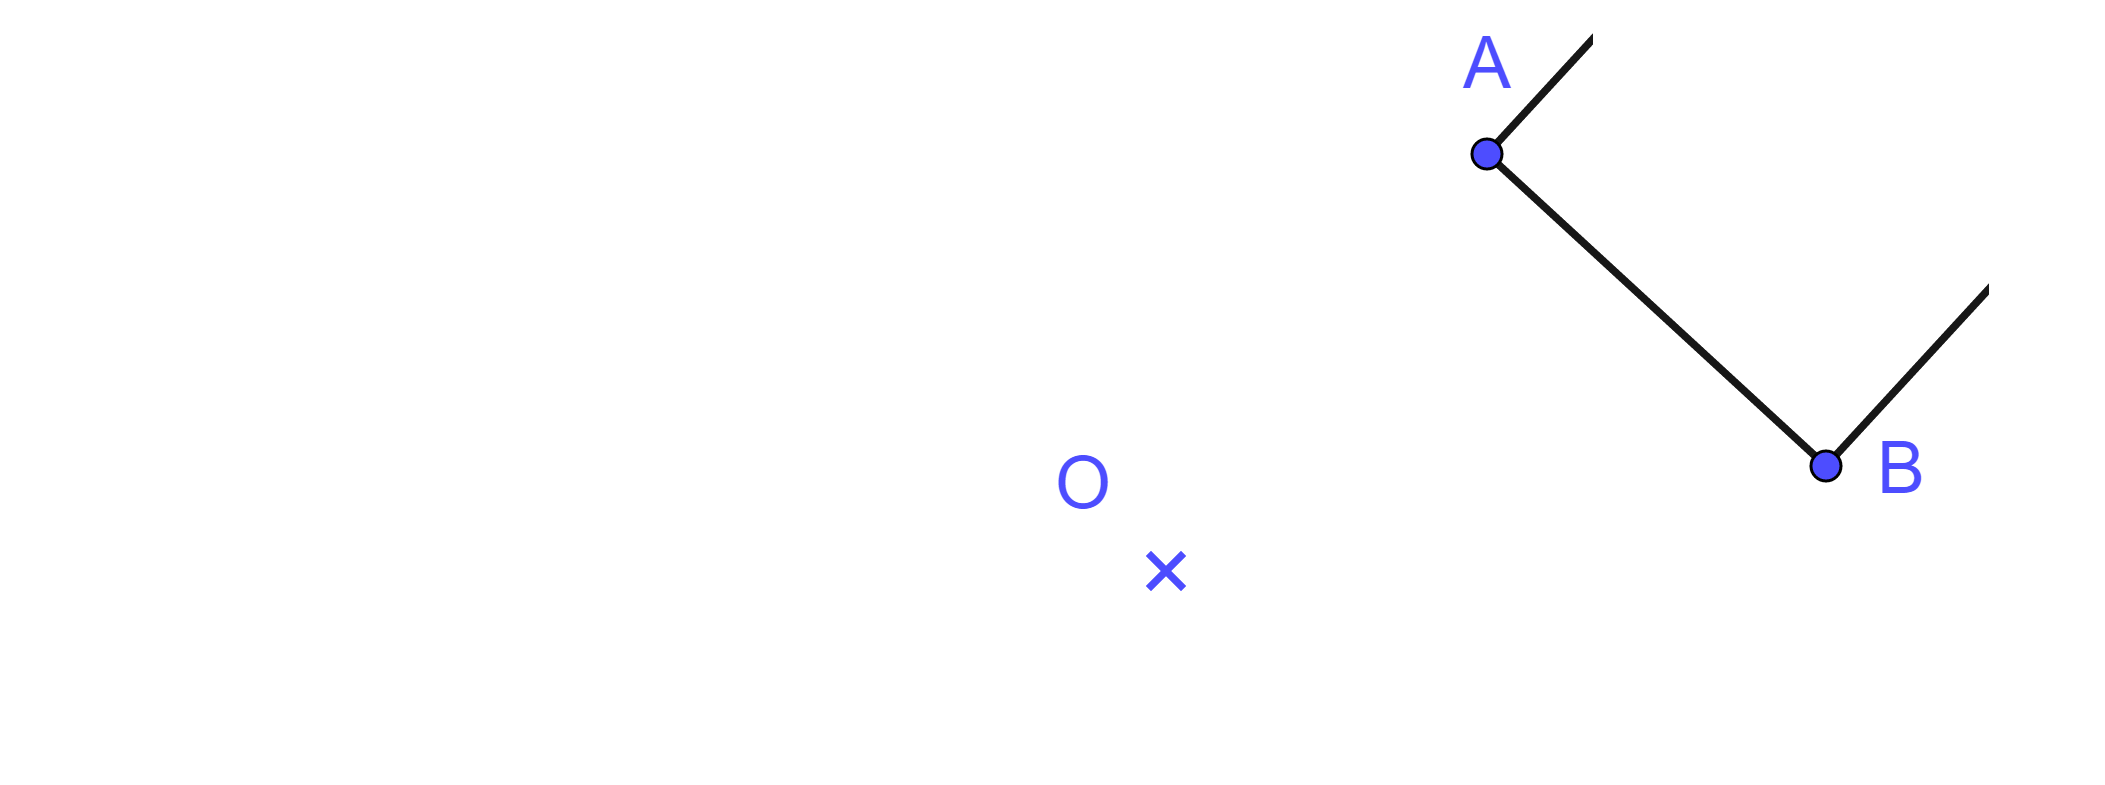
\includegraphics[scale=0.3]{img/carre}
	\end{center}

	\begin{solution}
		\begin{center}
			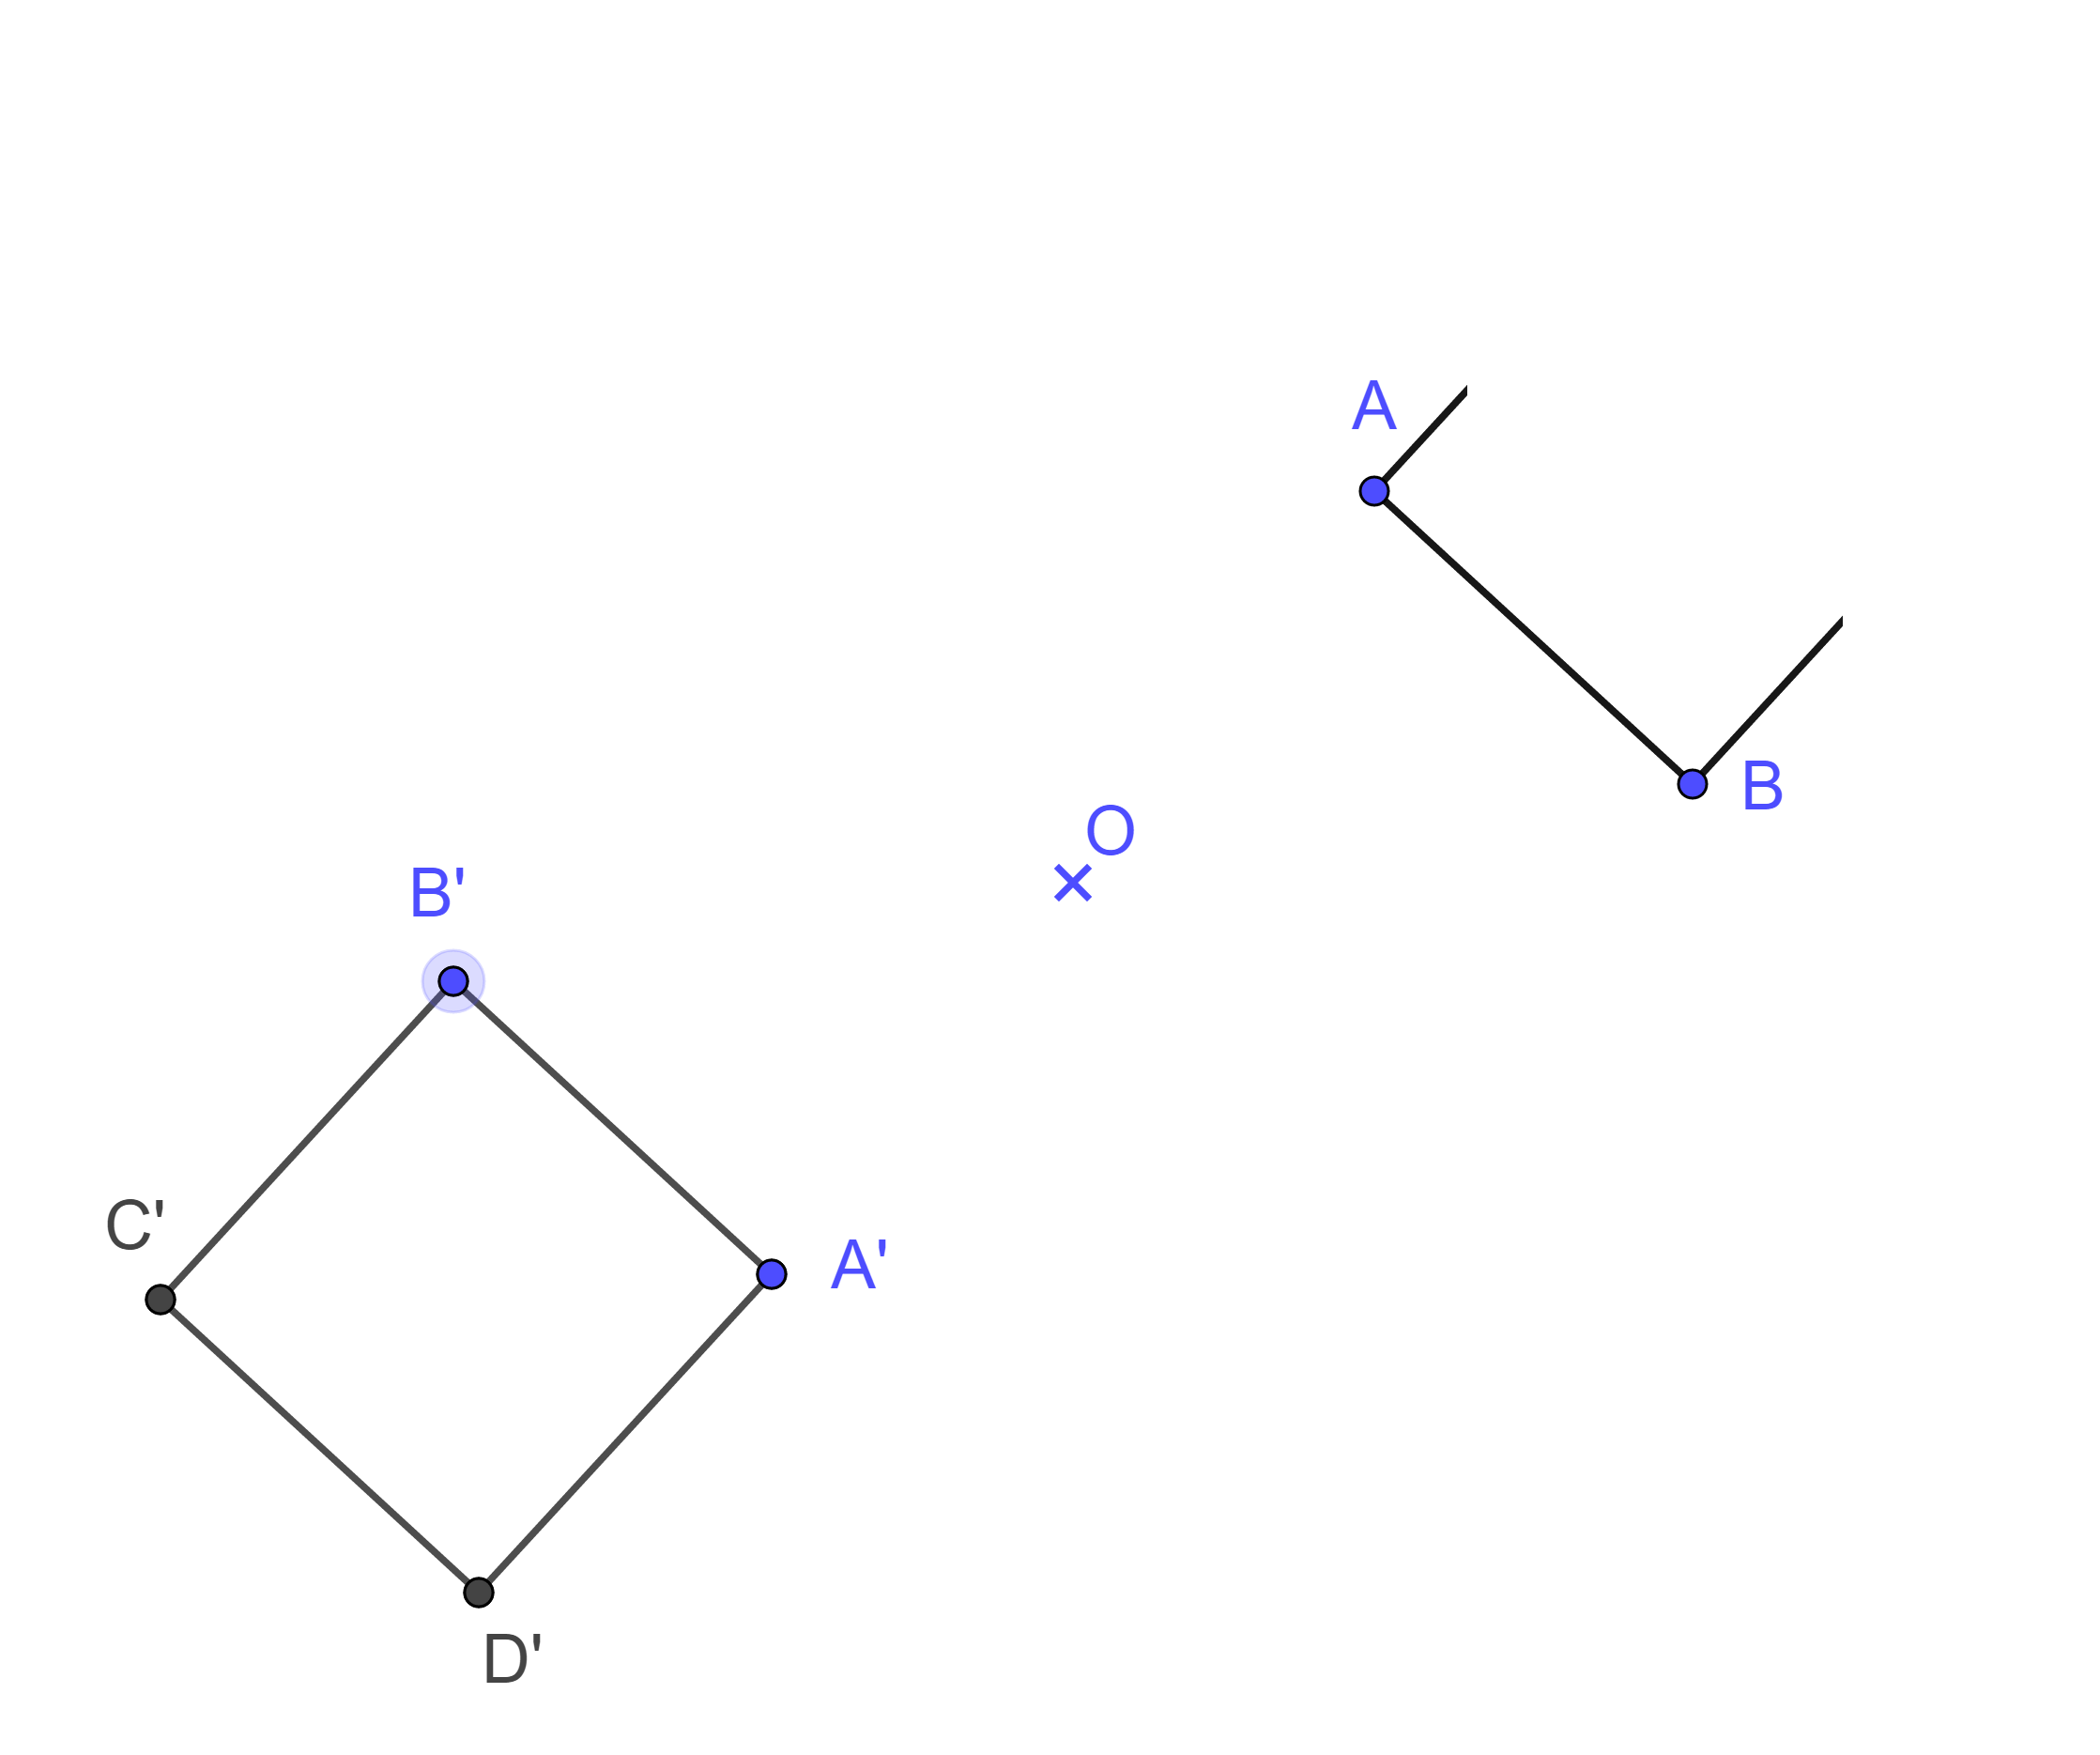
\includegraphics[scale=0.3]{img/carre_corr}
		\end{center}
	\end{solution}
\end{questions}

